\begin{figure}[!htbp]
\centering
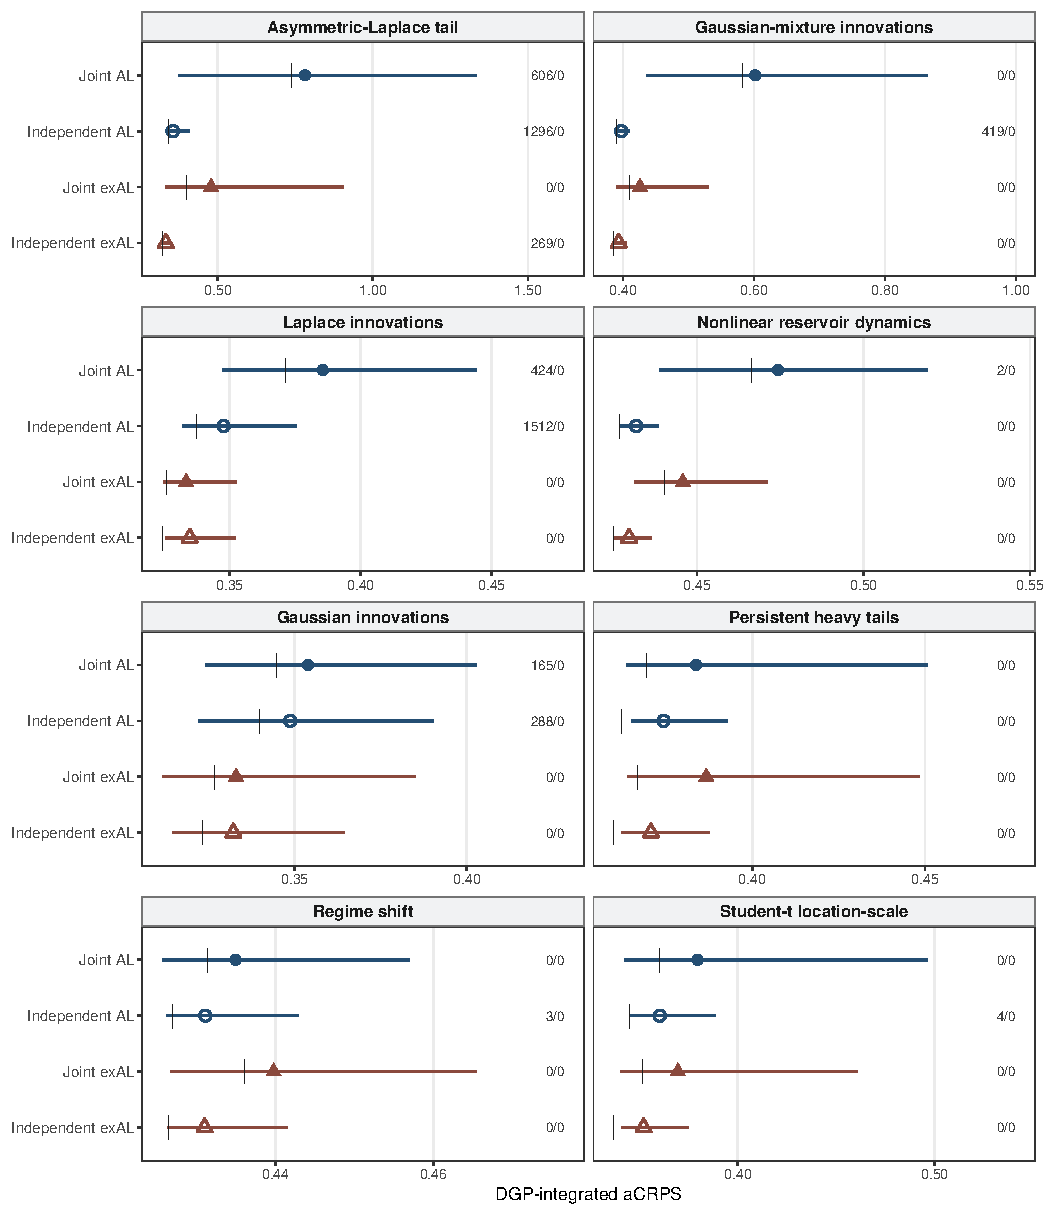
\includegraphics[width=0.94\textwidth]{figures/joint_qdesn_simulation/joint_qdesn_corrected_v4_forecast_dgp_acrps.pdf}
\caption{Corrected posterior DGP-integrated \(\aCRPS\) for the joint multi-quantile study. Colored points are posterior means and horizontal segments are equal-tailed 95\% intervals; black vertical marks give the canonical-action scores. Lower values are better. Filled symbols denote joint fits, open symbols independent fits, blue \(\AL\), and red \(\exAL\). Labels give raw/reported crossing counts for the canonical grid. All reported counts are zero after the pre-specified monotone rule. Marginal intervals for the numerical winner and runner-up overlap in every setting.}
\label{fig:joint-qdesn-corrected-v4-forecast-acrps}
\end{figure}
